\newcommand{\minipagespace}[1]{
	\begin{minipage}[c]{#1\textwidth}
		\ 
	\end{minipage}
}

\section{Culling}

Der erste Weg eine Voxel Engine zu optimieren wird
offensichtlich, wenn man sich einen Würfel aus $8$
Voxels betrachtet. Dabei beobachten wir, dass
die Hälfte der Seiten der Voxels nach innen schauen
und somit nicht sichtbar sind. Wenn man die
Seitenlänge dieses Würfels verdoppelt, multipliziert
man die Oberfläche mit $4$ und das Volumen mit $8$.
Somit entstehen immer mehr Seiten, die nach innen
schauen, umso größer das Objekt ist. Also wird
dies bei großen Objekten dazu führen, dass die
meisten Seiten nicht sichtbar sind.

\begin{center}
\begin{figure}[ht]
	\minipagespace{0.04}
	\begin{minipage}[c]{0.4\textwidth}
		\begin{center}
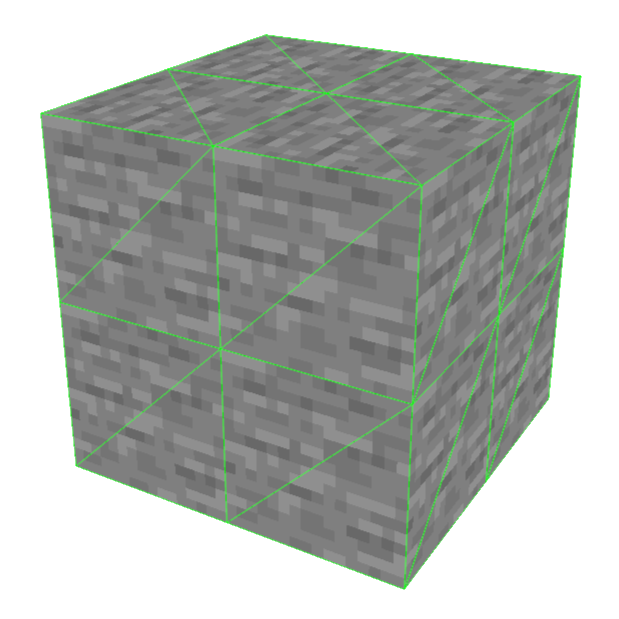
\includegraphics[width=1\textwidth]{assets/Culling/Opaque8Blocks.png}
		\end{center}
	\end{minipage}
	\minipagespace{0.09}
	\begin{minipage}[c]{0.4\textwidth}
		\begin{center}
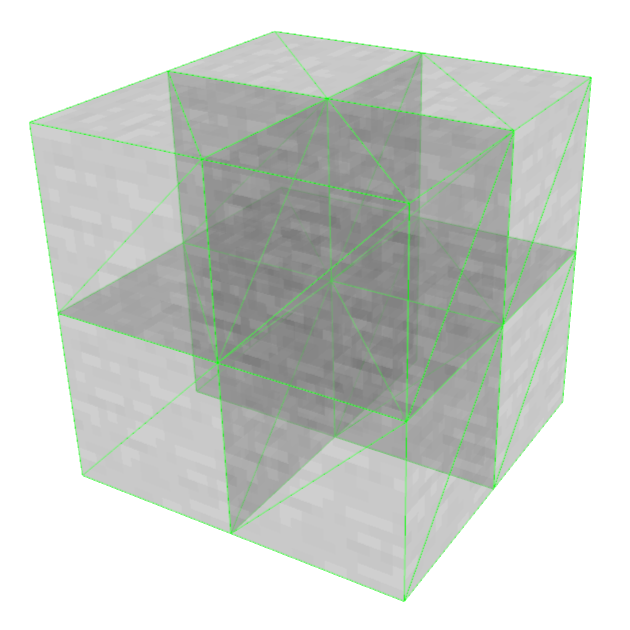
\includegraphics[width=1\textwidth]{assets/Culling/Transparent8Blocks.png}
		\end{center}
	\end{minipage}\hfill
\end{figure}
\end{center}

Mit \gqq{Culling} beschreibt man die Optimierung,
diese Seiten zu entfernen.

{ \subsection{Erste Implementation}

Die jetzige Methode ein Polygonnetz der Voxels
zu erstellen besteht darin, für jeden Voxel
ein Würfelnetz zu erstellen.
Um dies also zu cullen, überprüft man
noch die Nachbarvoxels, um zu entscheiden,
welche Seiten sichtbar sind, und erstellt nur
die sichtbaren Seiten.

% TODO maybe show some of the code here

Da die Spielwelt unendlich groß ist, muss sie
in viele einzelne Polygonnetze aufgeteilt werden.
Somit ist die Welt in sogenannte \gqq{Chunks}
eingeteilt, die $32 \times 32 \times 32$ Voxels
beinhalten. Das Polygonnetz, das die Voxels in einem
Chunk anzeigt, werde ich als
\gqq{Chunknetz} bezeichnen.

% TODO insert the image of chunk borders somewhere here

Da das Erstellen eines Chunknetzes lang dauern kann,
soll das Spiel nicht darauf warten,
da dies sonst sichtbar beim Spielen wäre.
Deswegen werden die Chunknetze in separaten
\href{https://de.wikipedia.org/wiki/Thread_(Informatik)}{Threads}
erstellt.
Zudem können somit mehrere Chunknetze gleichzeitig
erstellt werden.

\vspace{0.3cm}

% TODO transition into the benchmarks

% dont know how to get rid of this
% warning or what it means
% Erste Implementation stats from: bench 01
\benchgraph{1}{
	algo                   & blue       & red       \\
	Erste Implementation   & 12.834184  & 0.672563  \\
}

\vspace{0.3cm}

Dadurch entsteht aber ein neues Problem: \\
Wenn mehrere Threads zugriff auf die gleichen Daten
haben, muss dieser Zugriff synchronisiert werden,
da sonst eine
\href{https://de.wikipedia.org/wiki/Wettlaufsituation}{Wettlaufsituation}
(genauer gesagt ein Data Race) entstehen kann.
\footnote{\url{https://doc.rust-lang.org/nomicon/races.html}}
Durch diese Synchronisierung müsste aber jeder Zugriff
zu Chunks auf andere Threads warten, was das gesamte
Spiel langsamer machen würde. Deswegen werden die
Daten der nötigen Chunks zu dem Thread rüberkopiert,
was langsam ist, da es sich hier über sehr große Daten
handelt.

Culling braucht Information aus den benachbarten
Chunks, um zu entscheiden, ob die Ränder des Chunks
sichtbar sind. Somit müssen die 6 Nachbarchunks
auch zu dem Thread rüberkopiert werden, was sehr viele
Daten sind. Man könnte zwar nur die Voxels
rüberkopieren, die am Rand des Chunks sind,
aber wir werden gleich eine Methode sehen,
die dieses Problem und andere auf einmal löst.

\vspace{0.3cm}

Ein weiteres Problem besteht darin, dass dieser
Algorithmus für jeden Voxel noch die 6 Nachbarn
betrachten muss. Somit wird jeder Voxel 7-mal
betrachtet.
 }

{ \subsection{Binäres Culling}

Wir können beide Probleme der ersten Implementation
mit einer neuen Methode lösen.
Wir betrachten dabei eine Reihe von Voxels als einen
64-Bit Integer, wobei die einzelnen Bits darstellen,
ob sich dort ein Voxel befindet.
Es werden dabei 64 Bits gebraucht und nicht nur 32,
da man für das Culling auch wissen muss,
welche Voxels sich am Rand eines Chunks befinden,
und ein Chunk 32 Voxels lang ist.
Somit könnten die Voxels in einem Chunk
(und dem Rand) als ein 2 dimensionales
Array von 64-Bit Integers dargestellt werden,
wobei die 2 Dimensionen des Arrays die
$y$- und $z$-Achse darstellen und der Integer eine
Reihe von Voxels in der $x$-Achse darstellt.
Der Vorteil davon ist, dass wir somit in der
$x$-Achse binäre Arithmetik anwenden können für
das Culling, was sehr schnell ist.

% TODO better explanation
Beim Culling müssen wir die Seiten von
Voxels finden, die nicht von einem anderen Voxel
verdeckt werden.
Mit binärer Arithmetik geht dies jetzt sehr einfach:

\begin{lstlisting}[language=Rust]
fn find_faces(mask: u64) -> u32 {
	((mask & !(mask >> 1)) >> 1) as u32
}
\end{lstlisting}
%
Diese Funktion gibt eine Bitmaske für alle Voxels,
die von links sichtbar sind.
Dabei ist das \code{mask \& !(mask >> 1)} zuständig
die sichtbaren Seiten zu erkennen.
Definiert man also eine Funktion mit
\code{mask \& !(mask << 1)}, dann bekommt man alle,
die von rechts sichtbar sind.
Das \code{((..) >> 1) as u32} ist dann zuständig
die einzelnen Bits, die den Rand des Chunks beschreiben,
zu entfernen, da diese nicht mehr gebraucht sind.
Diese neue Bitmaske kann dann wie folgt verwendet
werden, um die Seiten der Voxels zu kreieren:

\begin{lstlisting}[language=Rust]
let mut mask = /* Bitmaske von dieser Reihe von Voxels */;
let mut k = 0;
while mask != 0 {
	let zeros = mask.trailing_zeros();
	mask = (mask >> zeros) & !1;
	k += zeros;
	// berechne die position dieser Seite basierend auf k,
	// und erstelle dann ein Mesh dafuer...
}
\end{lstlisting}

Um diese Funktion anwenden zu können, müssen
wir die Bitmaske aber erst konstruieren.
Dies werden wir für jede Achse wiederholen,
da jede Bitmaske nur für eine Achse anwendbar ist:

\begin{lstlisting}[language=Rust]
for (pos, block) in chunk.blocks.iter_xyz() {
	let BlockInChunkPos { x, y, z } = pos;
	let [x, y, z] = [x as usize, y as usize, z as usize];
	if block_models[&block.id].should_cull {
		blocks_mask[Axis::X][y][z] |= 1 << (x + 1);
		blocks_mask[Axis::Y][x][z] |= 1 << (y + 1);
		blocks_mask[Axis::Z][x][y] |= 1 << (z + 1);
	}
}
\end{lstlisting}

Dabei brauchen wir auch nur einen Zugriff pro Voxel,
während wir in der ersten Implementation 7 Zugriffe
pro Voxel brauchten.
Diese Bitmasken können wir erst erstellen und
dann dem neuen Thread rübersenden.

% TODO code of neighbour chunks

Insgesamt erhalten wir folgende Performance:

\vspace{0.3cm}

% Binäres Culling 1 stats from: bench 03
\benchgraph{2}{0.65}{
	algo                   & blue       & red       \\
	Erste Implementation   & 12.834184  & 0.672563  \\
	Binäres Culling 1      &  2.883930  & 5.155590  \\
}

\vspace{0.3cm}

Von 13,51 ms auf 8,04 ms ist eine Verbesserung
von 40,5 \%. Das sieht erstmal gut aus,
jedoch hat sich die Zeit einen neuen Thread zu
erstellen stark erhöht. Wir haben nämlich die Bitmaske
erst auf dem Main Thread
\footnote{Um genau zu sein, gibt es in Bevy
nicht einen \gqq{Main} Thread, wo die meisten Sachen
gemacht werden, sondern alles ist auf mehrere Threads
verteilt. Jedoch müssen alle
\href{https://bevy-cheatbook.github.io/programming/systems.html}{Systeme}
fertig sein, damit Bevy den nächsten Frame anzeigt,
und das wird hier blockiert.}
erstellt, damit nicht die
gesamten Daten des Chunks rübergesendet werden müssen.
Die Bitmaske zu erstellen braucht aber länger,
als den Chunk rüberzusenden.

Wir wollen, dass den Thread zu erstellen möglichst
schnell geht, da der Rest des Spiels warten muss,
bis dies fertig ist. Somit könnte die Performance
vom Spiel beeinträchtigt werden. Dieses Problem gibt
es nicht beim Erstellen des Chunk Meshes, da dies auf
einem separaten Thread passiert, was heißt, dass der
Chunk Mesh nicht in einem Frame generiert werden muss,
und somit die Performance nicht beeinflusst.

Obwohl es die gesamte Zeit den Chunk zu generieren
langsamer machen wird, werden wir deswegen die gesamten
Daten des Chunks und dessen Nachbarn an den neuen
Thread senden, der dann selbst eine Bitmaske erstellt.
Diesmal habe ich nicht die einfachere Implementation
benutzt, und habe wirklich nur den Rand rüberkopiert:

\begin{lstlisting}[language=Rust]
pub fn chunk_padding_from_neighbour_chunks(
	neighbours: FaceMap<&Chunk>
) -> ChunkPadding {
	let mut chunk_padding = FaceMap::from_map(|_|
		[[Air::BLOCK; CHUNK_LENGTH]; CHUNK_LENGTH]
	);

	macro_rules! axes {
		($(($a:ident, $b:ident) in ($axis:expr, $axis_name:ident)
		=> [$x:expr, $y:expr, $z:expr]);* $(;)?) => {
			$(
			for $a in 0..CHUNK_LENGTH {
				for $b in 0..CHUNK_LENGTH {
					let mut pos = BlockInChunkPos::new($x, $y, $z);

					pos.$axis_name = CHUNK_LENGTH as u8 - 1;
					let block = neighbours[$axis.face_neg()].blocks[pos];
					chunk_padding[$axis.face_neg()][$a][$b] = block;

					pos.$axis_name = 0;
					let block = neighbours[$axis.face_pos()].blocks[pos];
					chunk_padding[$axis.face_pos()][$a][$b] = block;
				}
			}
			)*
		};
	}
	axes! {
		(y, z) in (Axis::X, x) => [0, y as u8, z as u8];
		(x, z) in (Axis::Y, y) => [x as u8, 0, z as u8];
		(x, y) in (Axis::Z, z) => [x as u8, y as u8, 0];
	}
	chunk_padding
}
\end{lstlisting}

Mit dieser Methode wird die Zeit viel mehr auf den
separaten Thread verschoben, während die gesamte
Zeit nur gering erhöht wurde:

\vspace{0.3cm}

% Binäres Culling 2 stats from: bench 07
\benchgraph{3}{0.4}{
	algo                   & blue       & red       \\
	Erste Implementation   & 12.834184  & 0.672563  \\
	Binäres Culling 1      &  2.883930  & 5.155590  \\
	Binäres Culling 2      &  8.524388  & 0.448866  \\
}
 }
